\documentclass[aspectratio=169]{beamer}

\usepackage[utf8]{inputenc}
\usepackage{tikz}
\usepackage{caption} % Per le caption
\usepackage{subcaption} % Per caption immagini
\usepackage{media9}  % Supporto media per gif
% \usetheme[darkmode, showmaxslides]{pureminimalistic}
% argomenti:
% - showmaxslides: nel footer, mostra pagina corrente / pagine totali. Se non utilizzato, solo pagina corrente
% - nofooterlogo: non mostra il logo nel footer
\usetheme[showmaxslides]{pureminimalistic}

\usepackage[doi=false, maxbibnames=2, maxcitenames=2,%
            style=numeric, sorting=none, url=false, eprint=false]{biblatex}
\addbibresource{bibliografia-tesi-Taiwo-Solomon.bib}
% this makes it possible to add backup slides, without counting them
\usepackage{appendixnumberbeamer}
\renewcommand{\appendixname}{\texorpdfstring{\translate{appendix}}{appendix}}

% presenter name
\newcommand{\presenter}{Taiwo Solomon Olamide}
% to define the conference name
% \newcommand{\conference}{}

\title[Gestione permessi]{Interfaccia web per la gestione dei permessi in una piattaforma E-learning per scuole superiori}
\author{Laureando: \textbf{Solomon Olamide Taiwo}\newline Relatore: \textbf{Prof. Fabrizio Riguzzi}\newline Secondo relatore: \textbf{Dr. Ing. Arnaud Nguembang Fadja}}
% \subtitle[Sottotitolo Abbreviato]{Sottotitolo Intero}
\institute{\newline Università degli Studi di Ferrara}
\date{Venerdì 12 Luglio 2024}

\begin{document}
% has to be loaded outside of a frame to work!
\maketitle

% For longer table of contents, I find it cleaner to
% use no footline.
% \begin{frame}[plain, noframenumbering]{Outline}
%	\tableofcontents
% \end{frame}

\section{Introduzione}
\begin{frame}[fragile]{Introduzione}
	\begin{columns}[T] % align columns at the top
		\begin{column}{0.65\textwidth}
			System Afrik Information Technology (SYAIT) è una realtà di origini ferraresi che ho aiutato, durante i mesi di tirocinio,
			nella realizzazione di un modulo per la gestione dei permessi degli utenti utilizzatori di una piattaforma E-learning.
		\end{column}
		\begin{column}{0.35\textwidth}
			\begin{figure}[H]
				\centering
				
\includegraphics[width=\textwidth]{../images/logo-syait.png}
			\end{figure}
		\end{column}
	\end{columns}

\end{frame}

\section{Requisiti del progetto}
\begin{frame}{Requisiti funzionali e non funzionali}
	\begin{columns}[T] % align columns at the top
		\begin{column}{0.5\textwidth}
			\textbf{Requisiti funzionali}
			\begin{itemize}
				\item \textbf{Creazione} dei componenti che visualizzano risorse e azioni
				\item \textbf{Realizzazione} del layout della pagina principale
				\item \textbf{Gestione} dei permessi
				\item \textbf{Accesso} alle funzionalità
			\end{itemize}
		\end{column}
		\begin{column}{0.5\textwidth}
			\textbf{Requisiti non funzionali}
			\begin{itemize}
				\item \textbf{Prestazioni} adeguate e costanti
				\item \textbf{Sicurezza}: best practises per realizzazione software sicuro
				\item \textbf{Usabilità}: applicativo facile da usare
				\item \textbf{Manutenibilità} del codice
			\end{itemize}
		\end{column}
	\end{columns}
\end{frame}

\begin{frame}[fragile]{Diagramma dei casi d'uso}
	\begin{figure}[H]
		\centering
		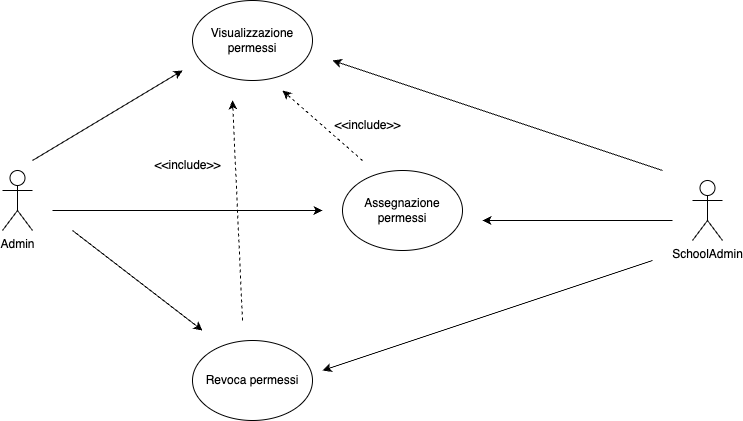
\includegraphics[width=0.7\textwidth]{../images/diagramma-casi-uso-attori.png}
	\end{figure}
\end{frame}

\section{Tecnologie utilizzate}
\begin{frame}{Tecnologie utilizzate}
	\begin{tikzpicture}[overlay, remember picture]
		\node at (1.5, 0) {
\includegraphics[width=0.3\textwidth]{../images/ruby-logo.png}};
		\node at (4.7, 0) {
\includegraphics[width=0.2\textwidth]{../images/rails-logo.png}};
		\node at (7.9, 0) {
\includegraphics[width=0.14\textwidth]{../images/postgresql-logo.png}};
		\node at (10.5, 0) {
\includegraphics[width=0.11\textwidth]{../images/vue.js-logo.png}};
		\node at (13, 0) {
\includegraphics[width=0.15\textwidth]{../images/quasar-logo.png}};
	\end{tikzpicture}
\end{frame}

\section{Implementazione della gestione dei permessi utente}

\subsection{Frontend e backend}

\begin{frame}[fragile]{Frontend e backend}
	\begin{columns}[T] % align columns at the top
		\begin{column}{0.5\textwidth}
			\textbf{Frontend}
			\begin{enumerate}
				\item \textbf{Design adottato}: utilizzo di mockup
				\item \textbf{Implementazione}: creazione componenti e implementazione in pagina frontend "Permissions"
			\end{enumerate}
		\end{column}
		\begin{column}{0.5\textwidth}
			\textbf{Backend}
			\begin{enumerate}
				\item \textbf{Schema} del database
				\item \textbf{Inizializzazione} del database
				\item \textbf{Implementazione}: modelli user e school e controller user
			\end{enumerate}
		\end{column}
	\end{columns}
\end{frame}

\begin{frame}[fragile]{Mockup del frontend}
	\begin{columns}[T] % align columns at the top
		\begin{column}{0.7\textwidth}
			\begin{figure}
				\centering
				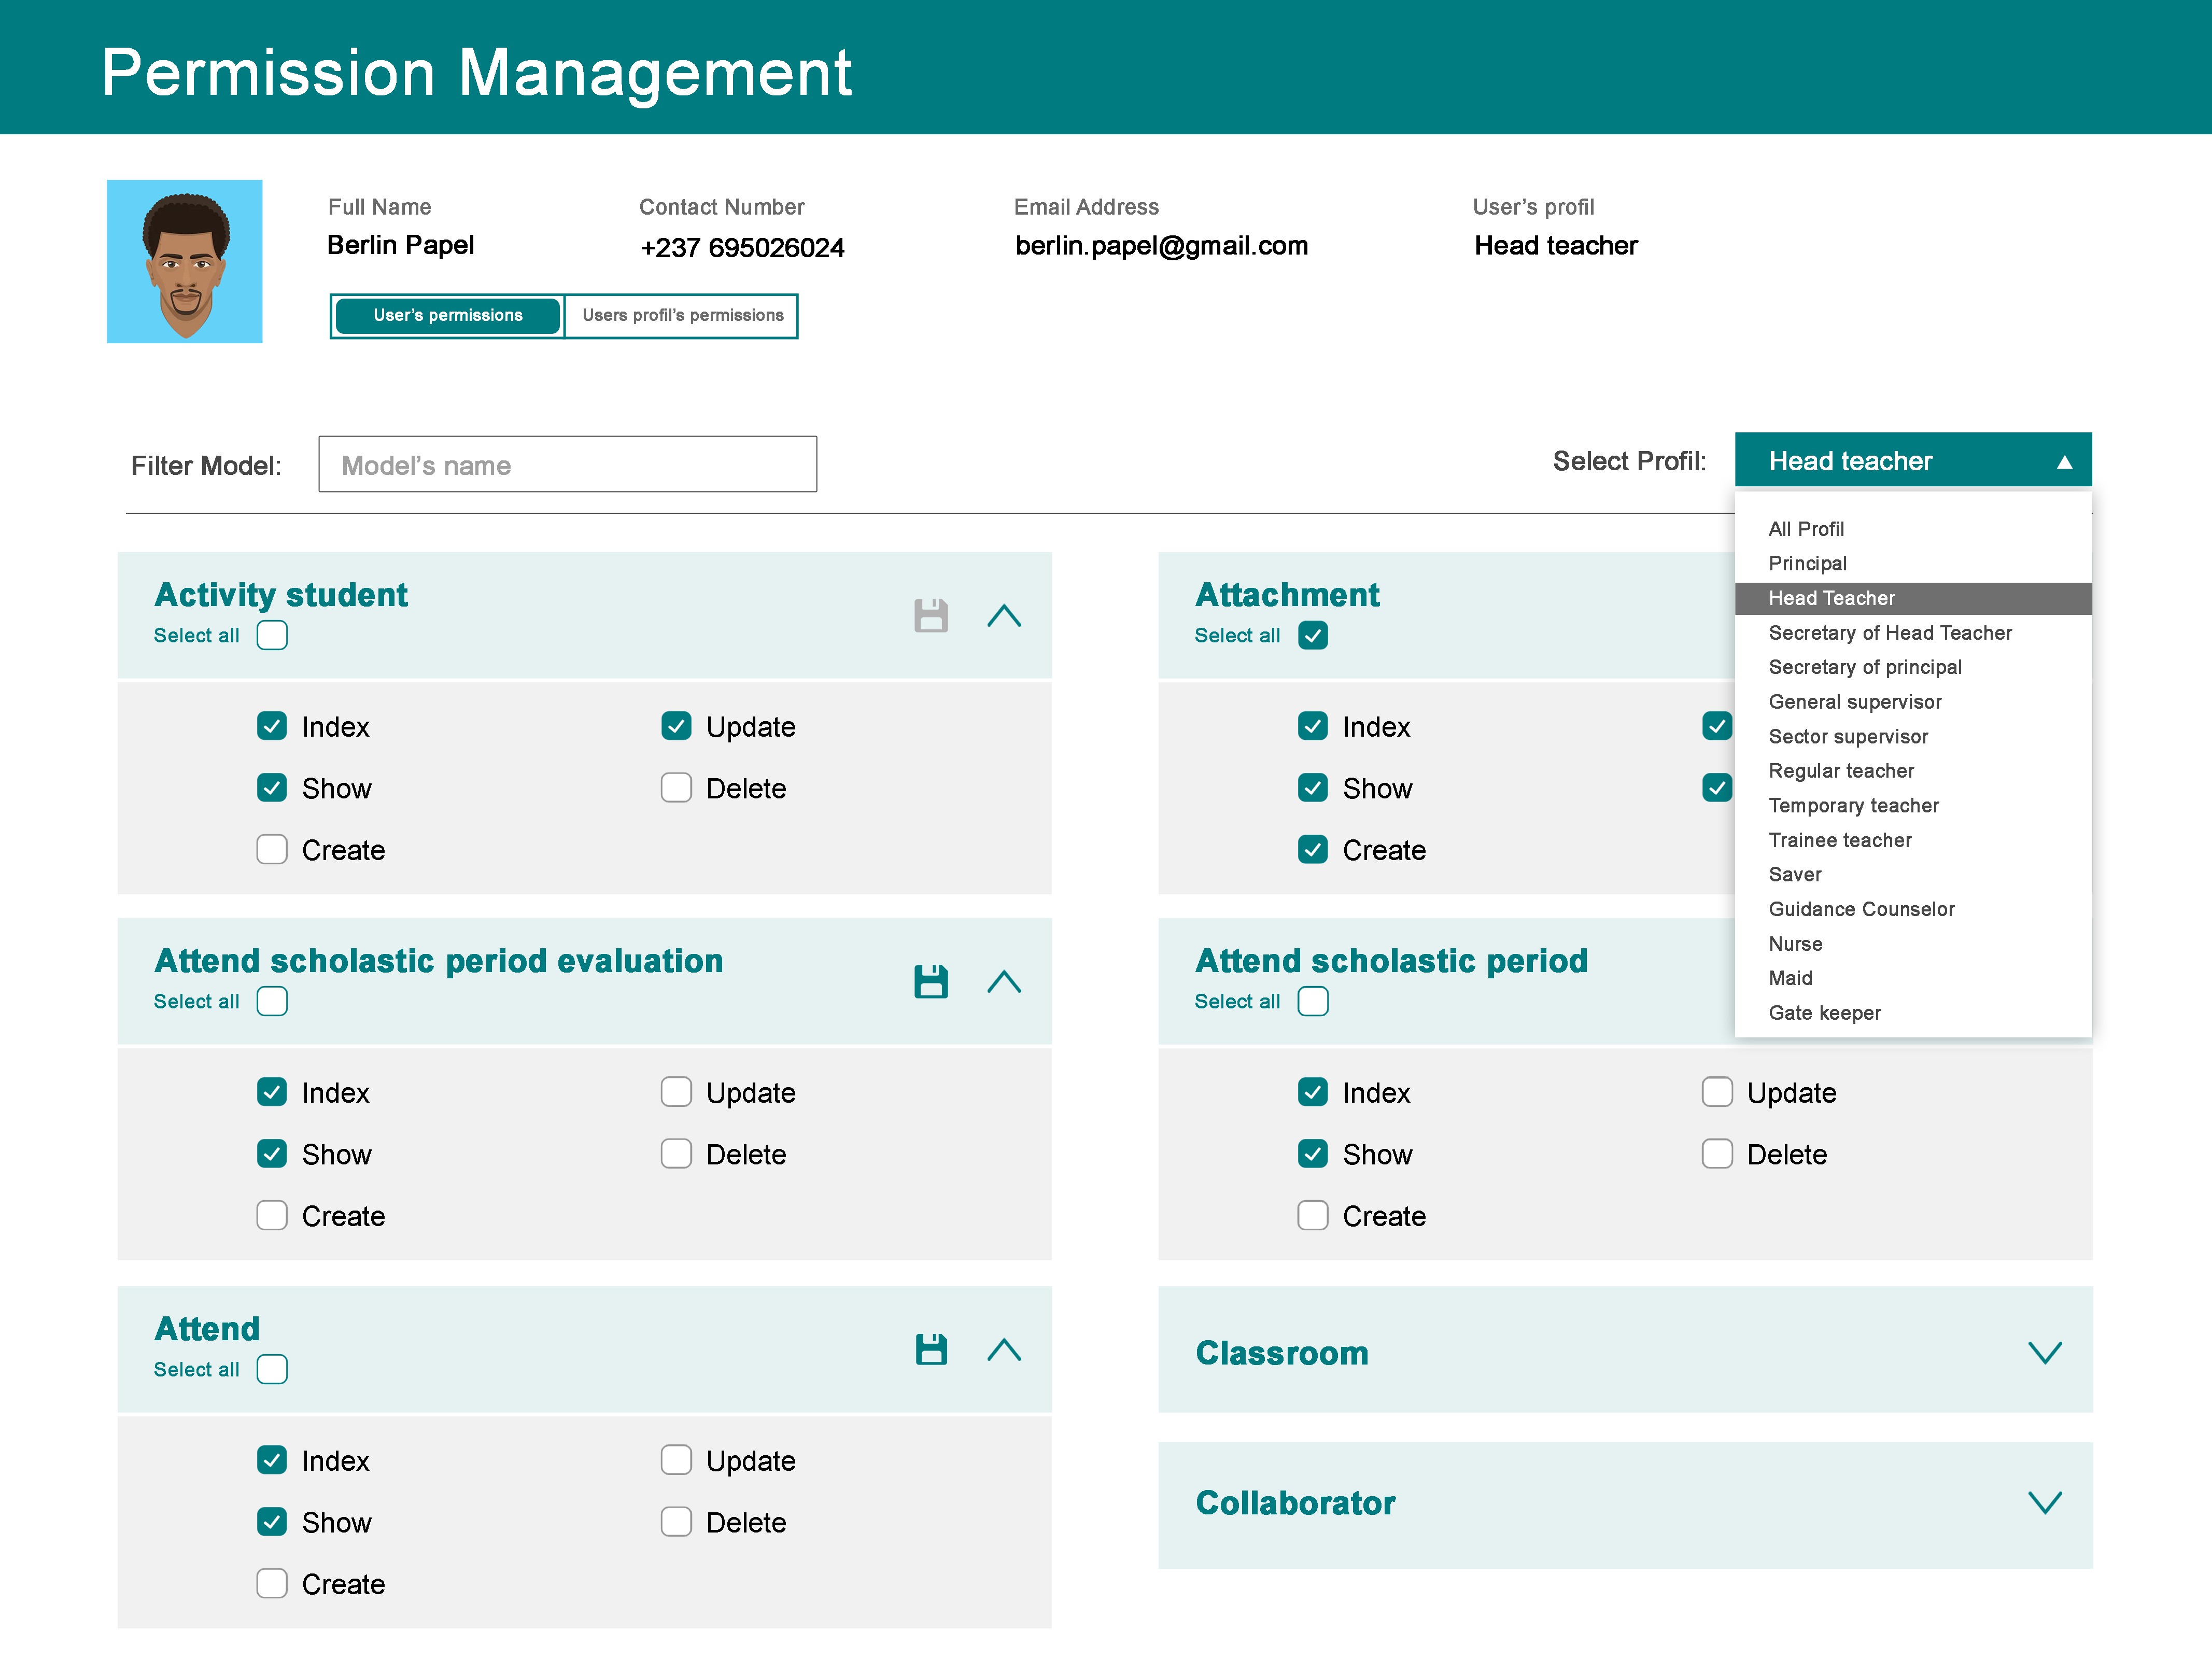
\includegraphics[width=0.85\textwidth]{../images/permission-management-desktop-mockup.jpg}
			\end{figure}
		\end{column}
		\begin{column}{0.3\textwidth}
			\begin{figure}
				\centering
				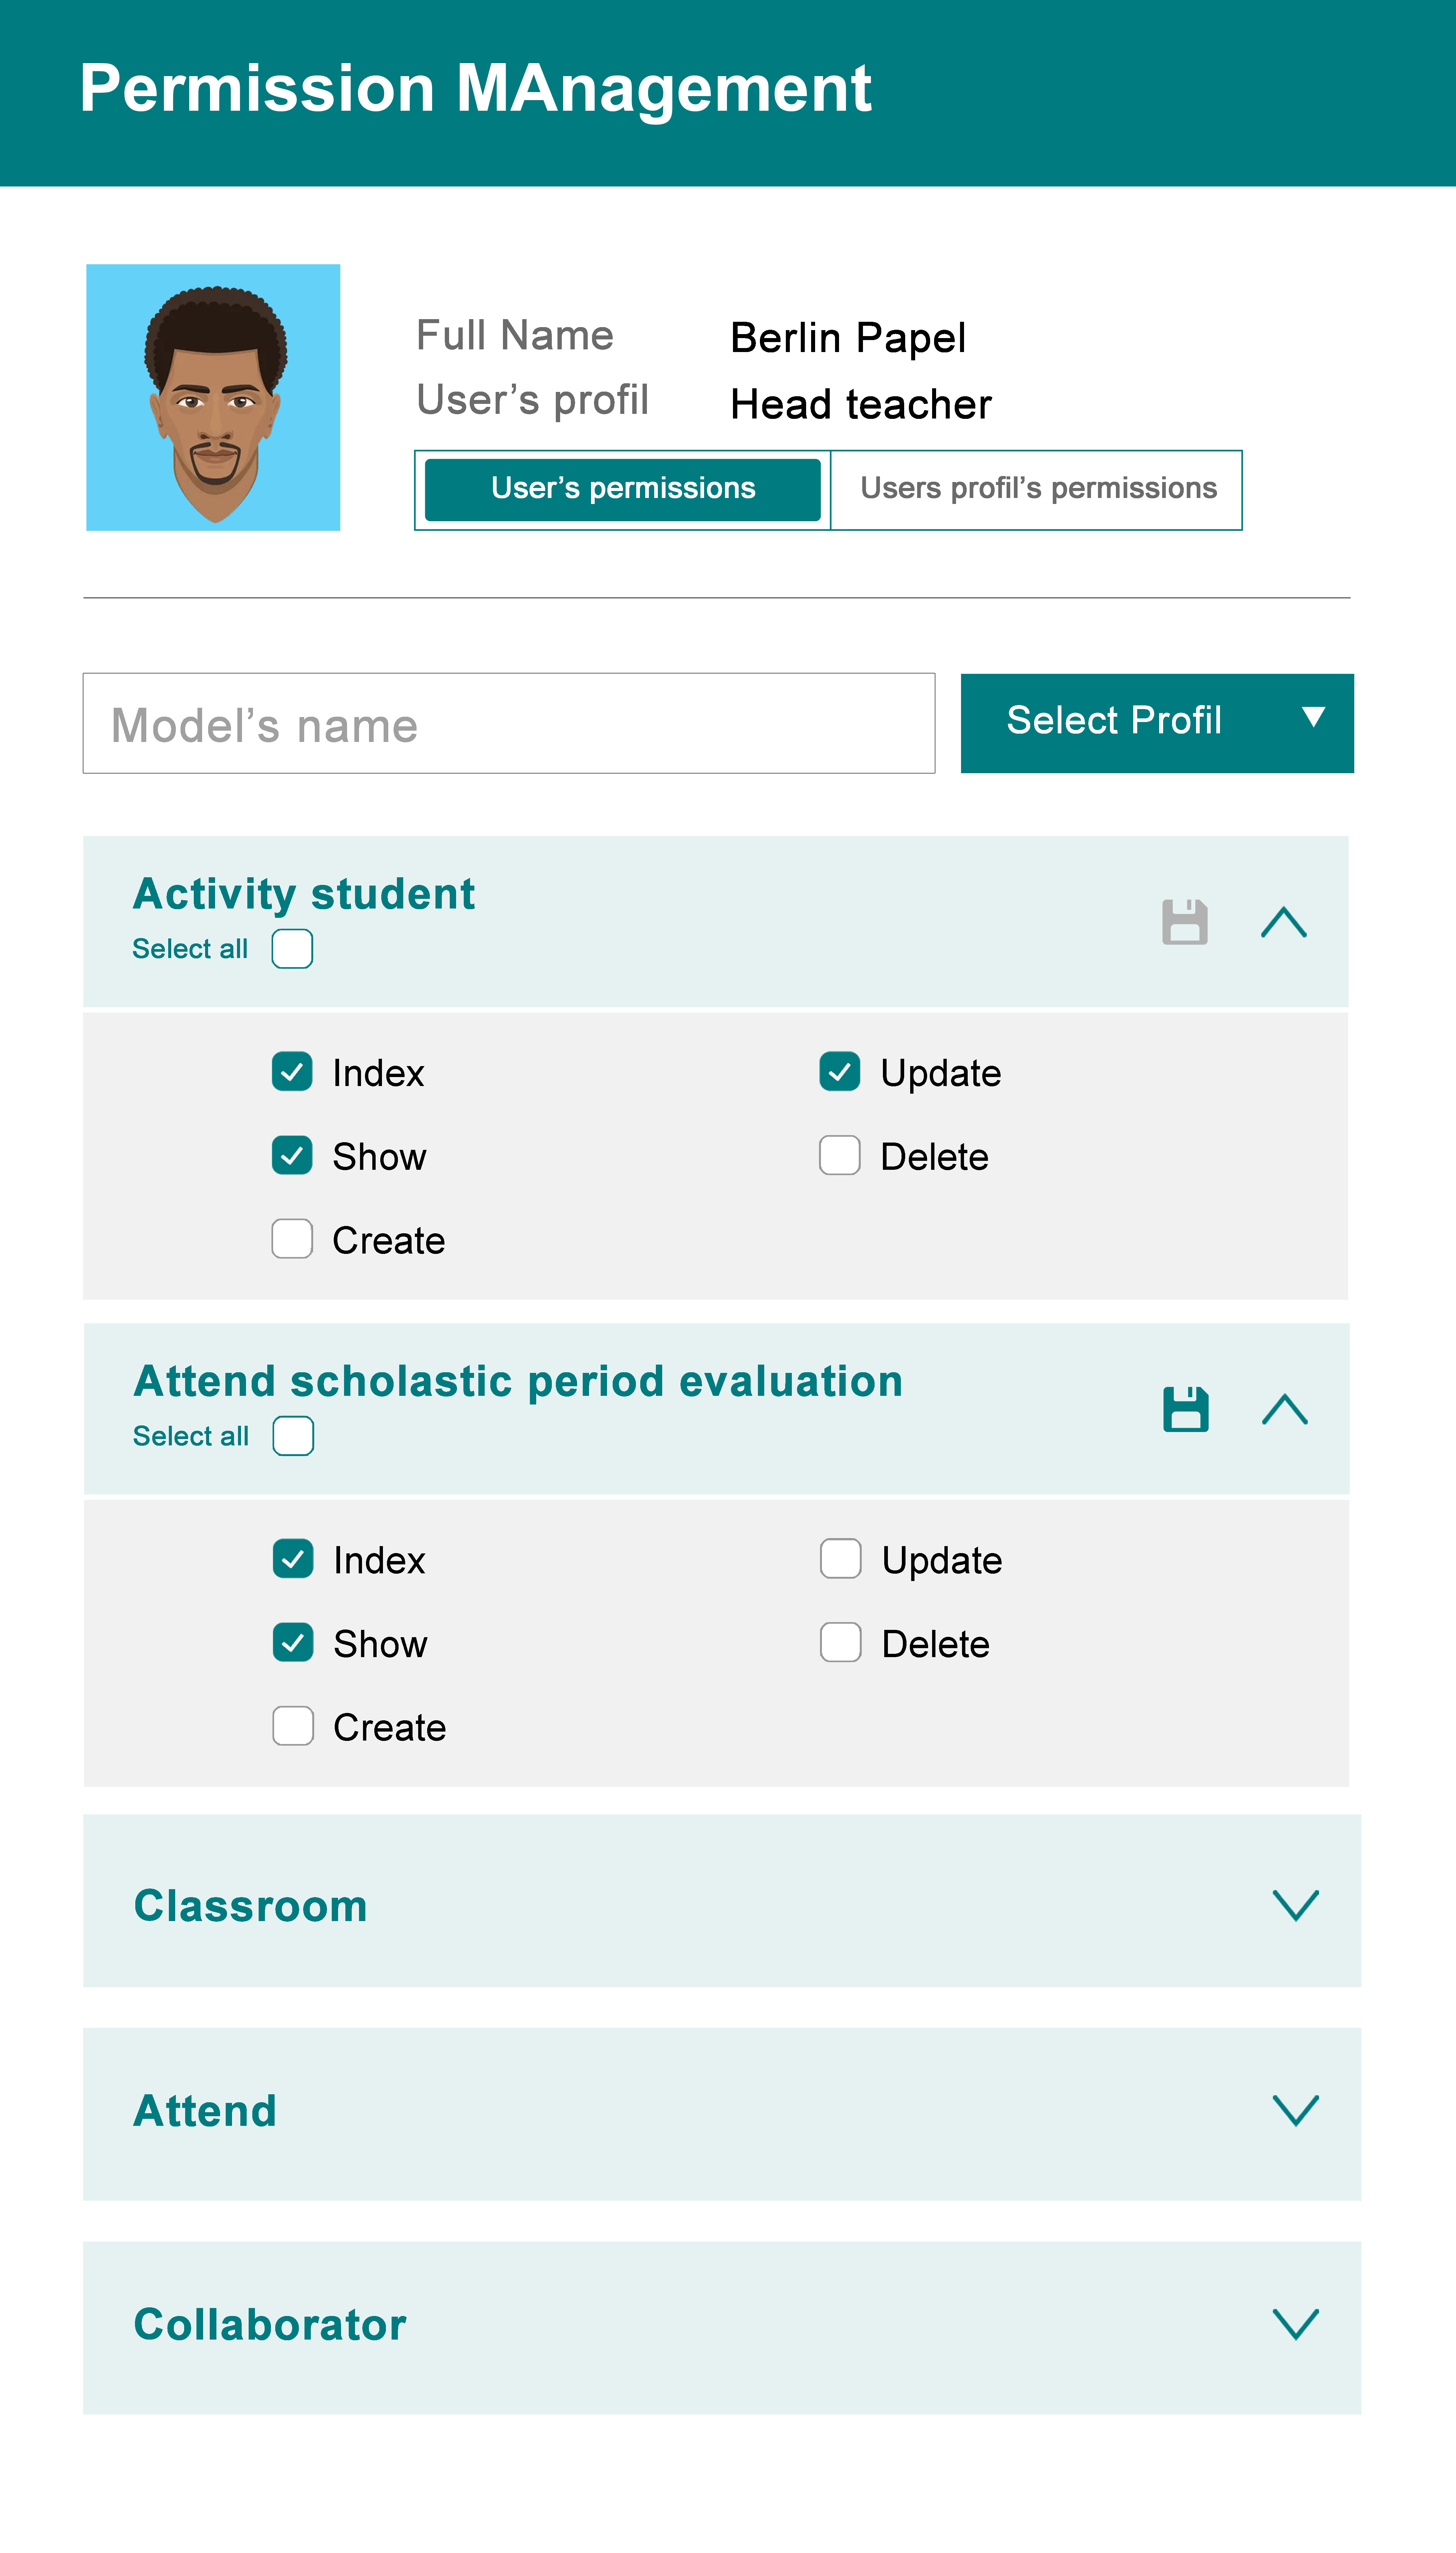
\includegraphics[width=0.85\textwidth]{../images/permission-management-mobile-mockup.jpg}
			\end{figure}
		\end{column}
	\end{columns}
\end{frame}

\subsection{Schemi relazionali}

\begin{frame}[fragile]{Schemi relazionali}
	\begin{figure}
		\centering
		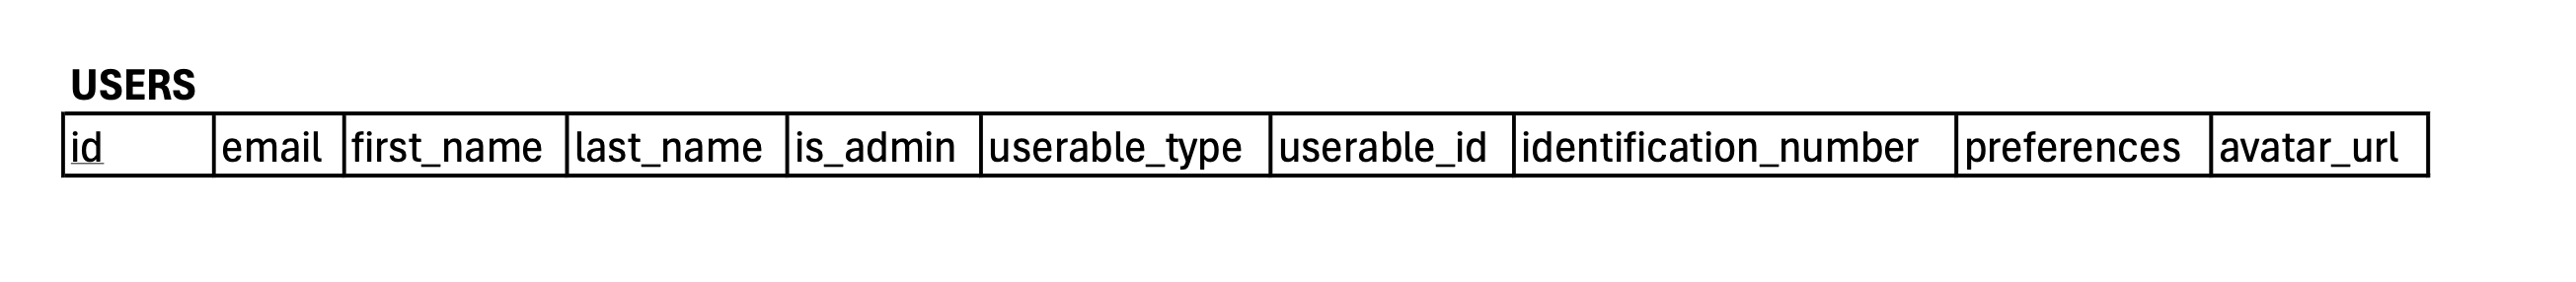
\includegraphics[width=\textwidth]{../images/schema-relazionale-users.png}
		
\includegraphics[width=\textwidth]{../images/schema-relazionale-schools.png}
	\end{figure}
\end{frame}

\begin{frame}[fragile]{Struttura del campo 'permissions' nella tabella 'schools'}
	\begin{figure}
		\centering
		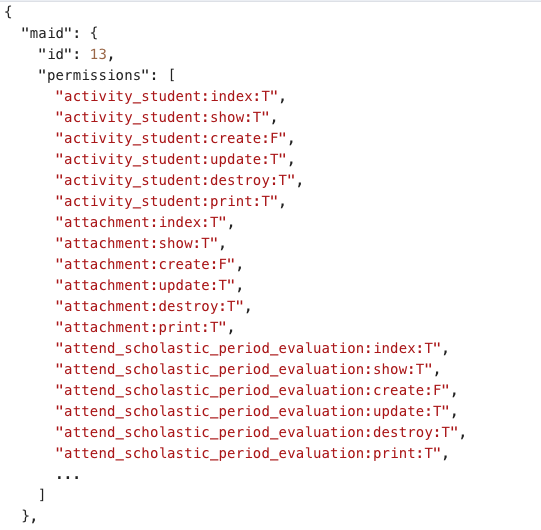
\includegraphics[width=0.4\textwidth]{../images/campo-permissions.png}
	\end{figure}
\end{frame}

\subsection{Implementazione frontend finale}

\begin{frame}[fragile]{Implementazione frontend finale - modifica permessi utente}
	\begin{columns}[T] % align columns at the top
		\begin{column}{0.7\textwidth}
			\begin{figure}
				\centering
				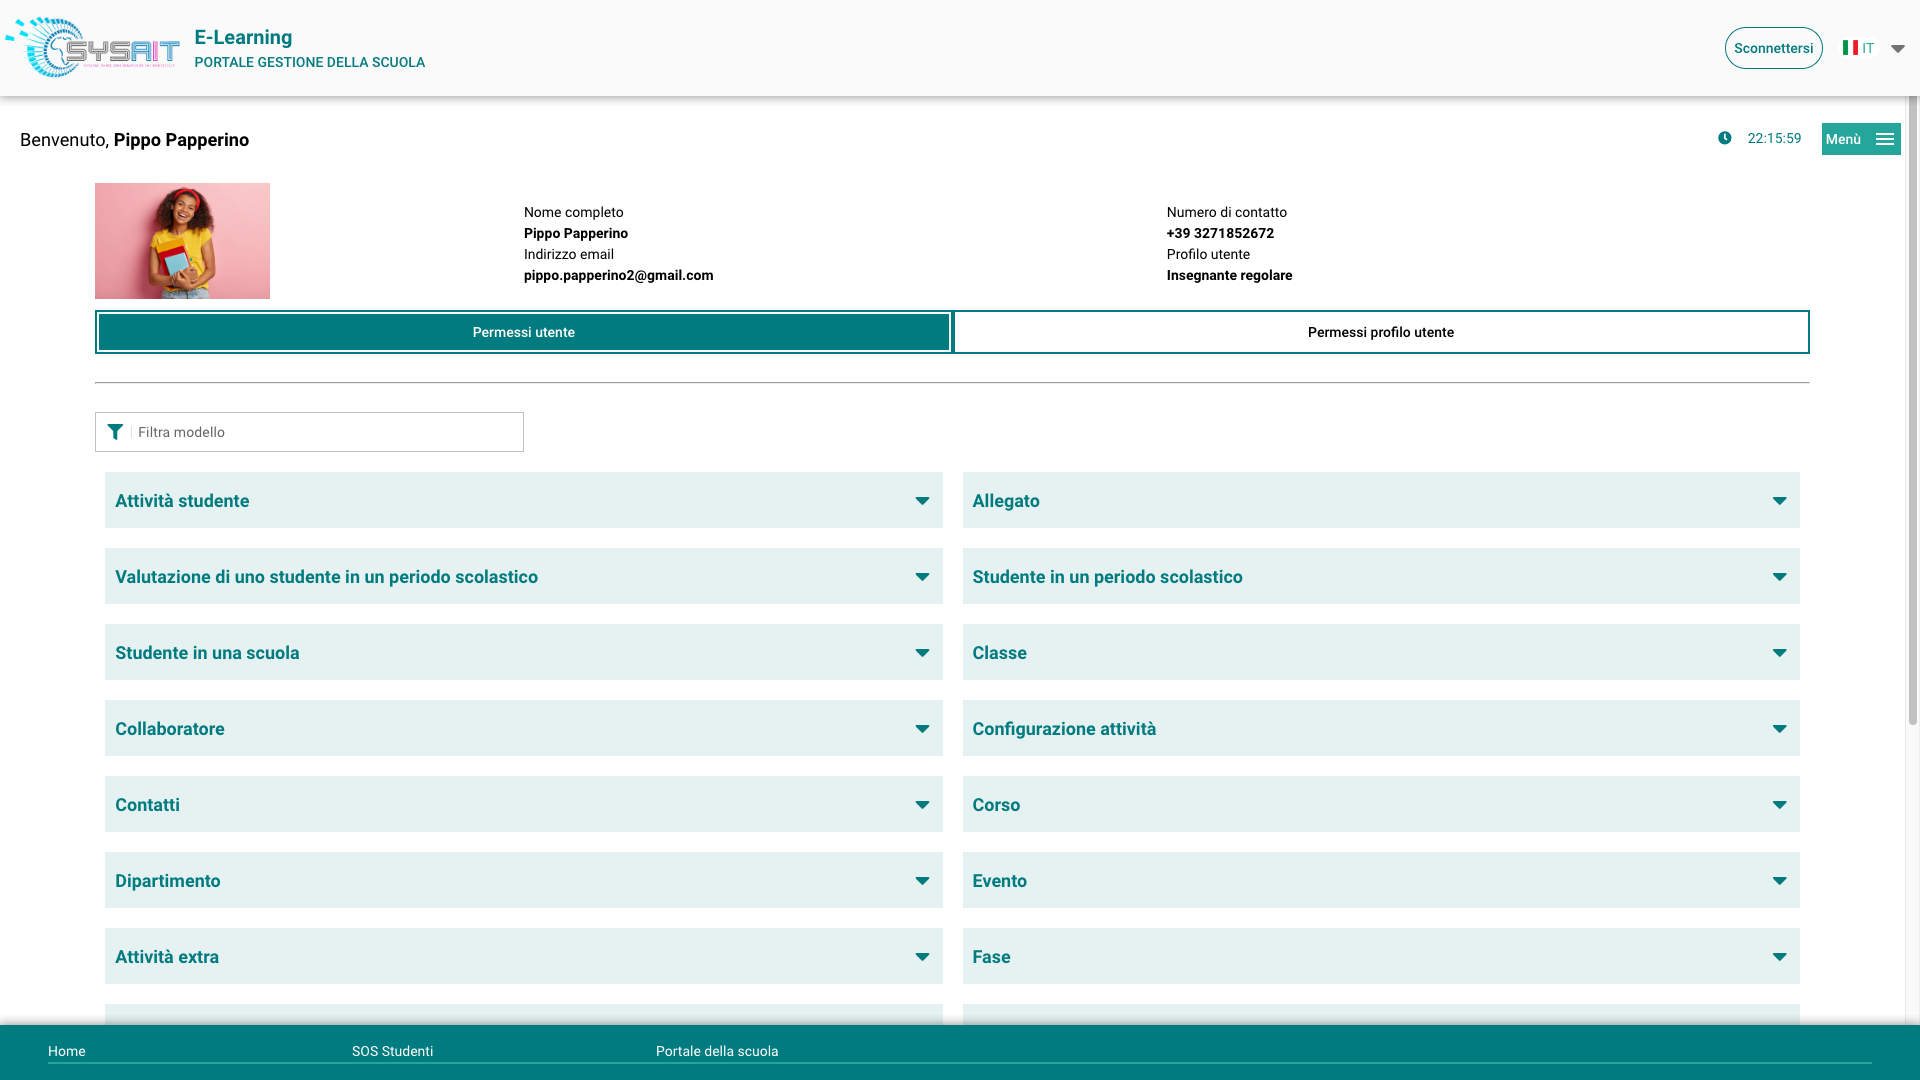
\includegraphics[width=\textwidth]{../images/permission-management-desktop.png}
			\end{figure}
		\end{column}
		\begin{column}{0.2\textwidth}
			\begin{figure}
				\centering
				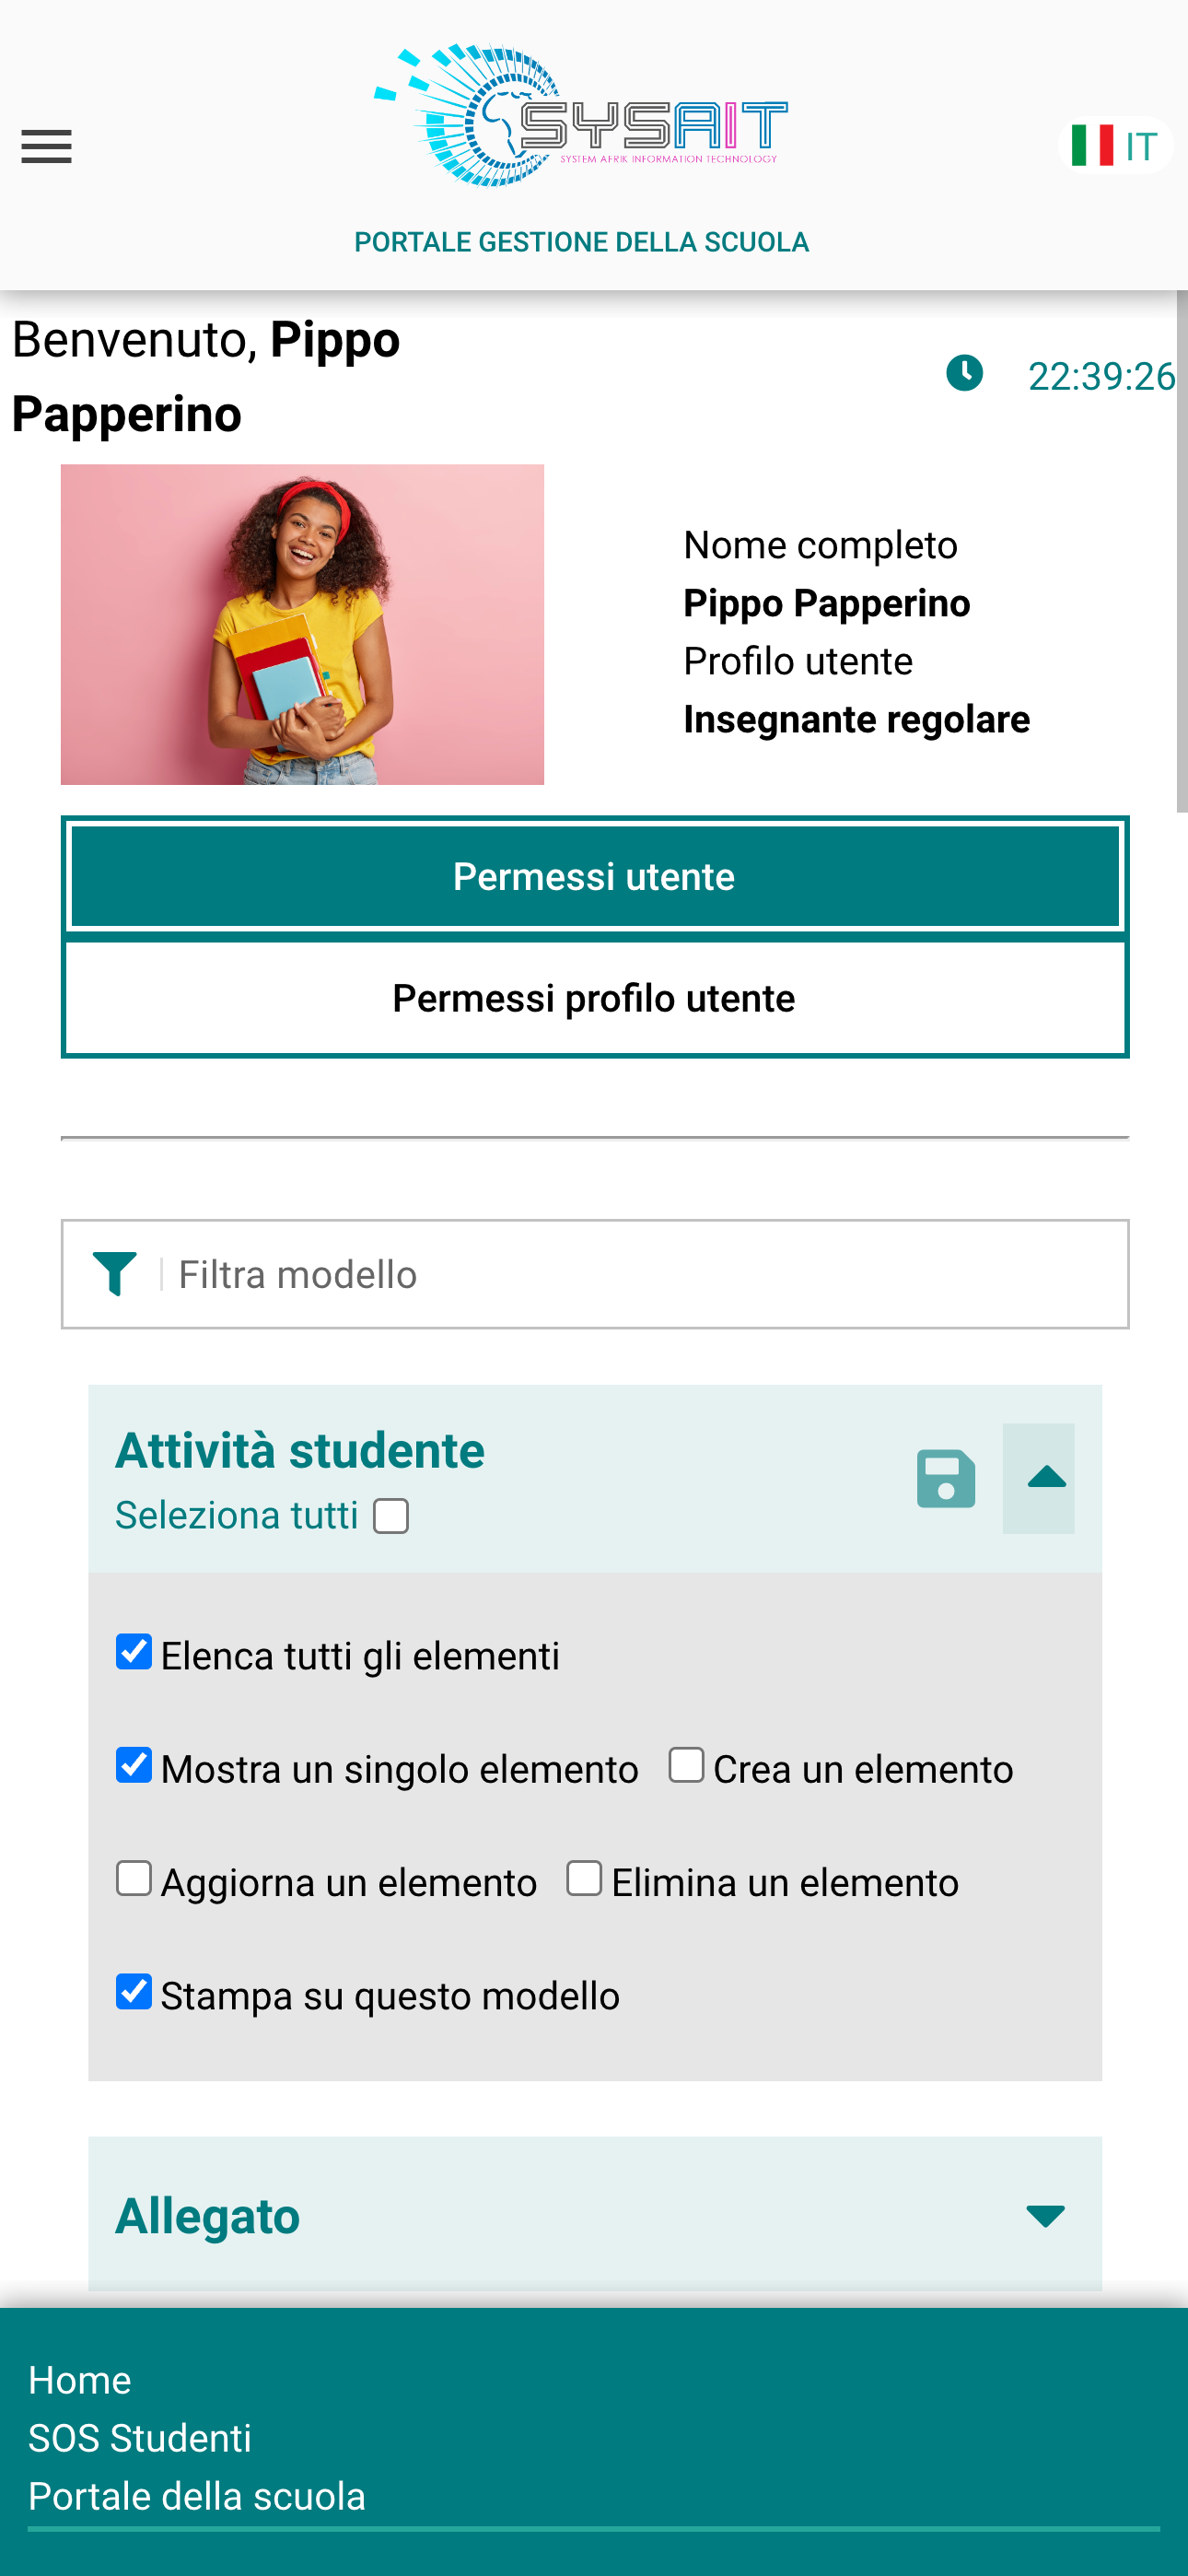
\includegraphics[width=0.9\textwidth]{../images/permission-management-mobile.png}
			\end{figure}
		\end{column}
	\end{columns}
\end{frame}

\begin{frame}[fragile]{Implementazione frontend finale - modifica permessi profilo}
	\begin{columns}[T]
		\begin{column}{0.7\textwidth}
			\begin{figure}
				\centering
				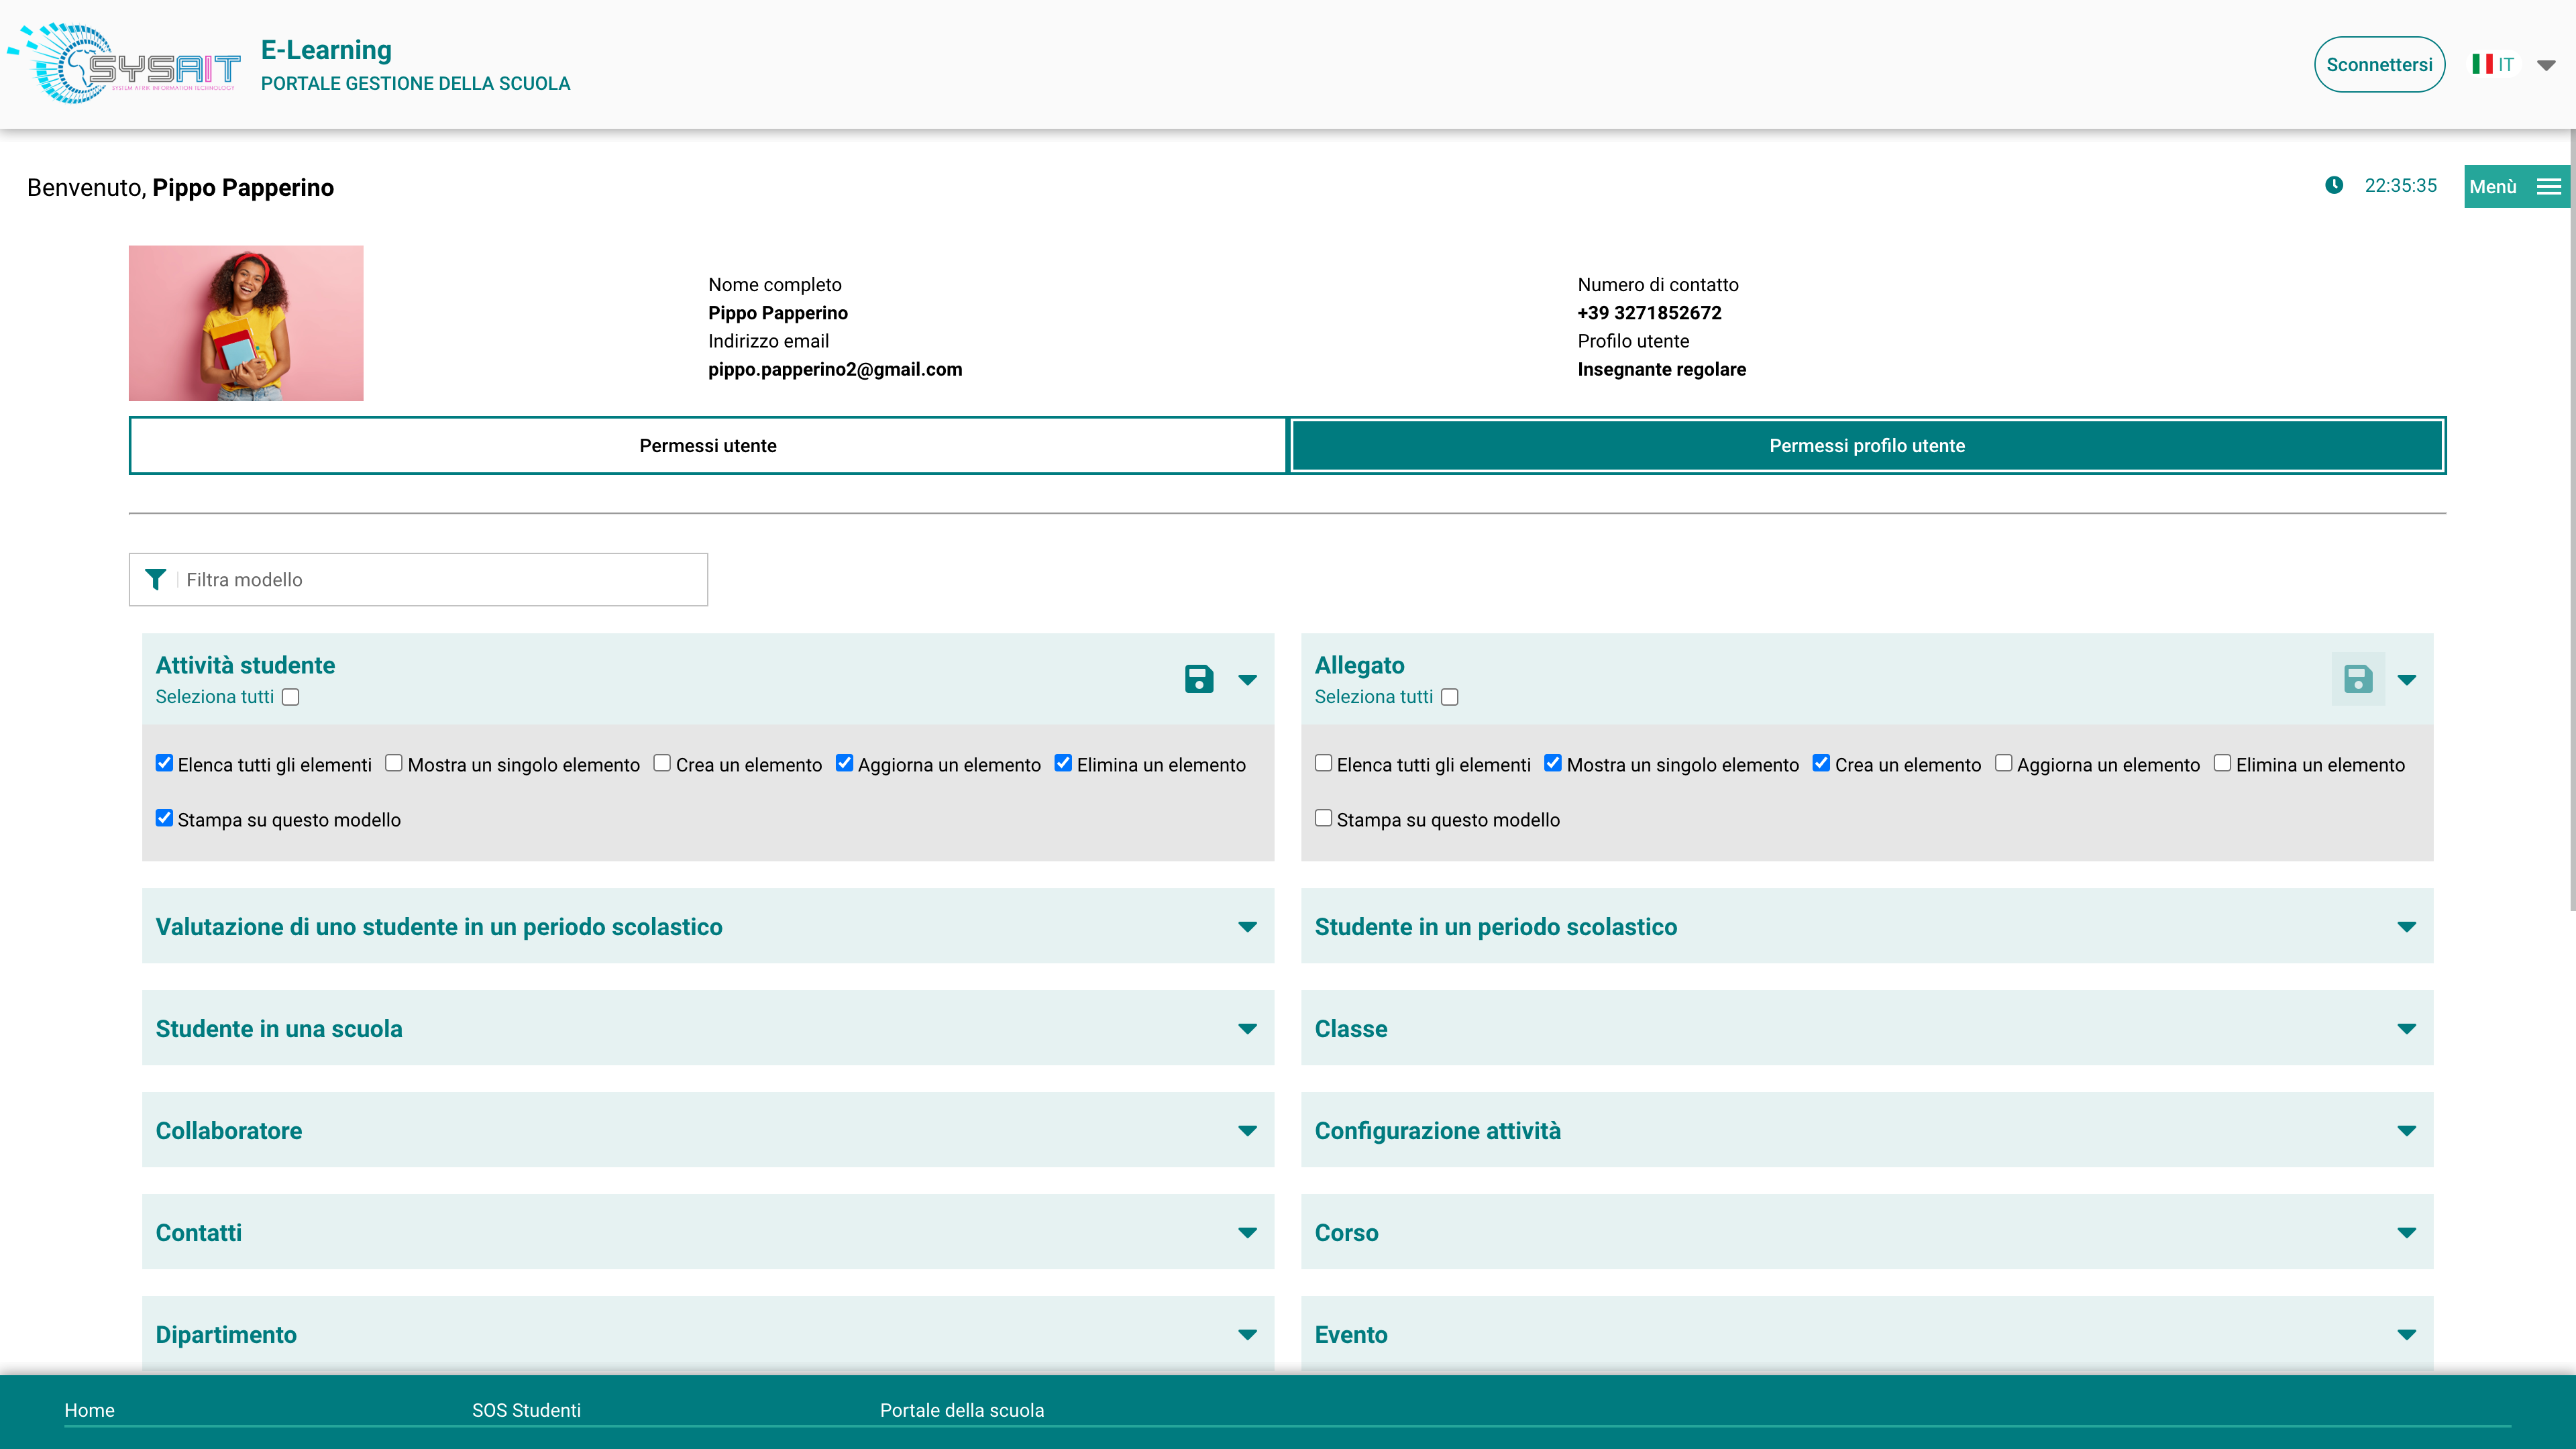
\includegraphics[width=\textwidth]{../images/permission-management-desktop-profile.png}
			\end{figure}
		\end{column}
		\begin{column}{0.2\textwidth}
			\begin{figure}
				\centering
				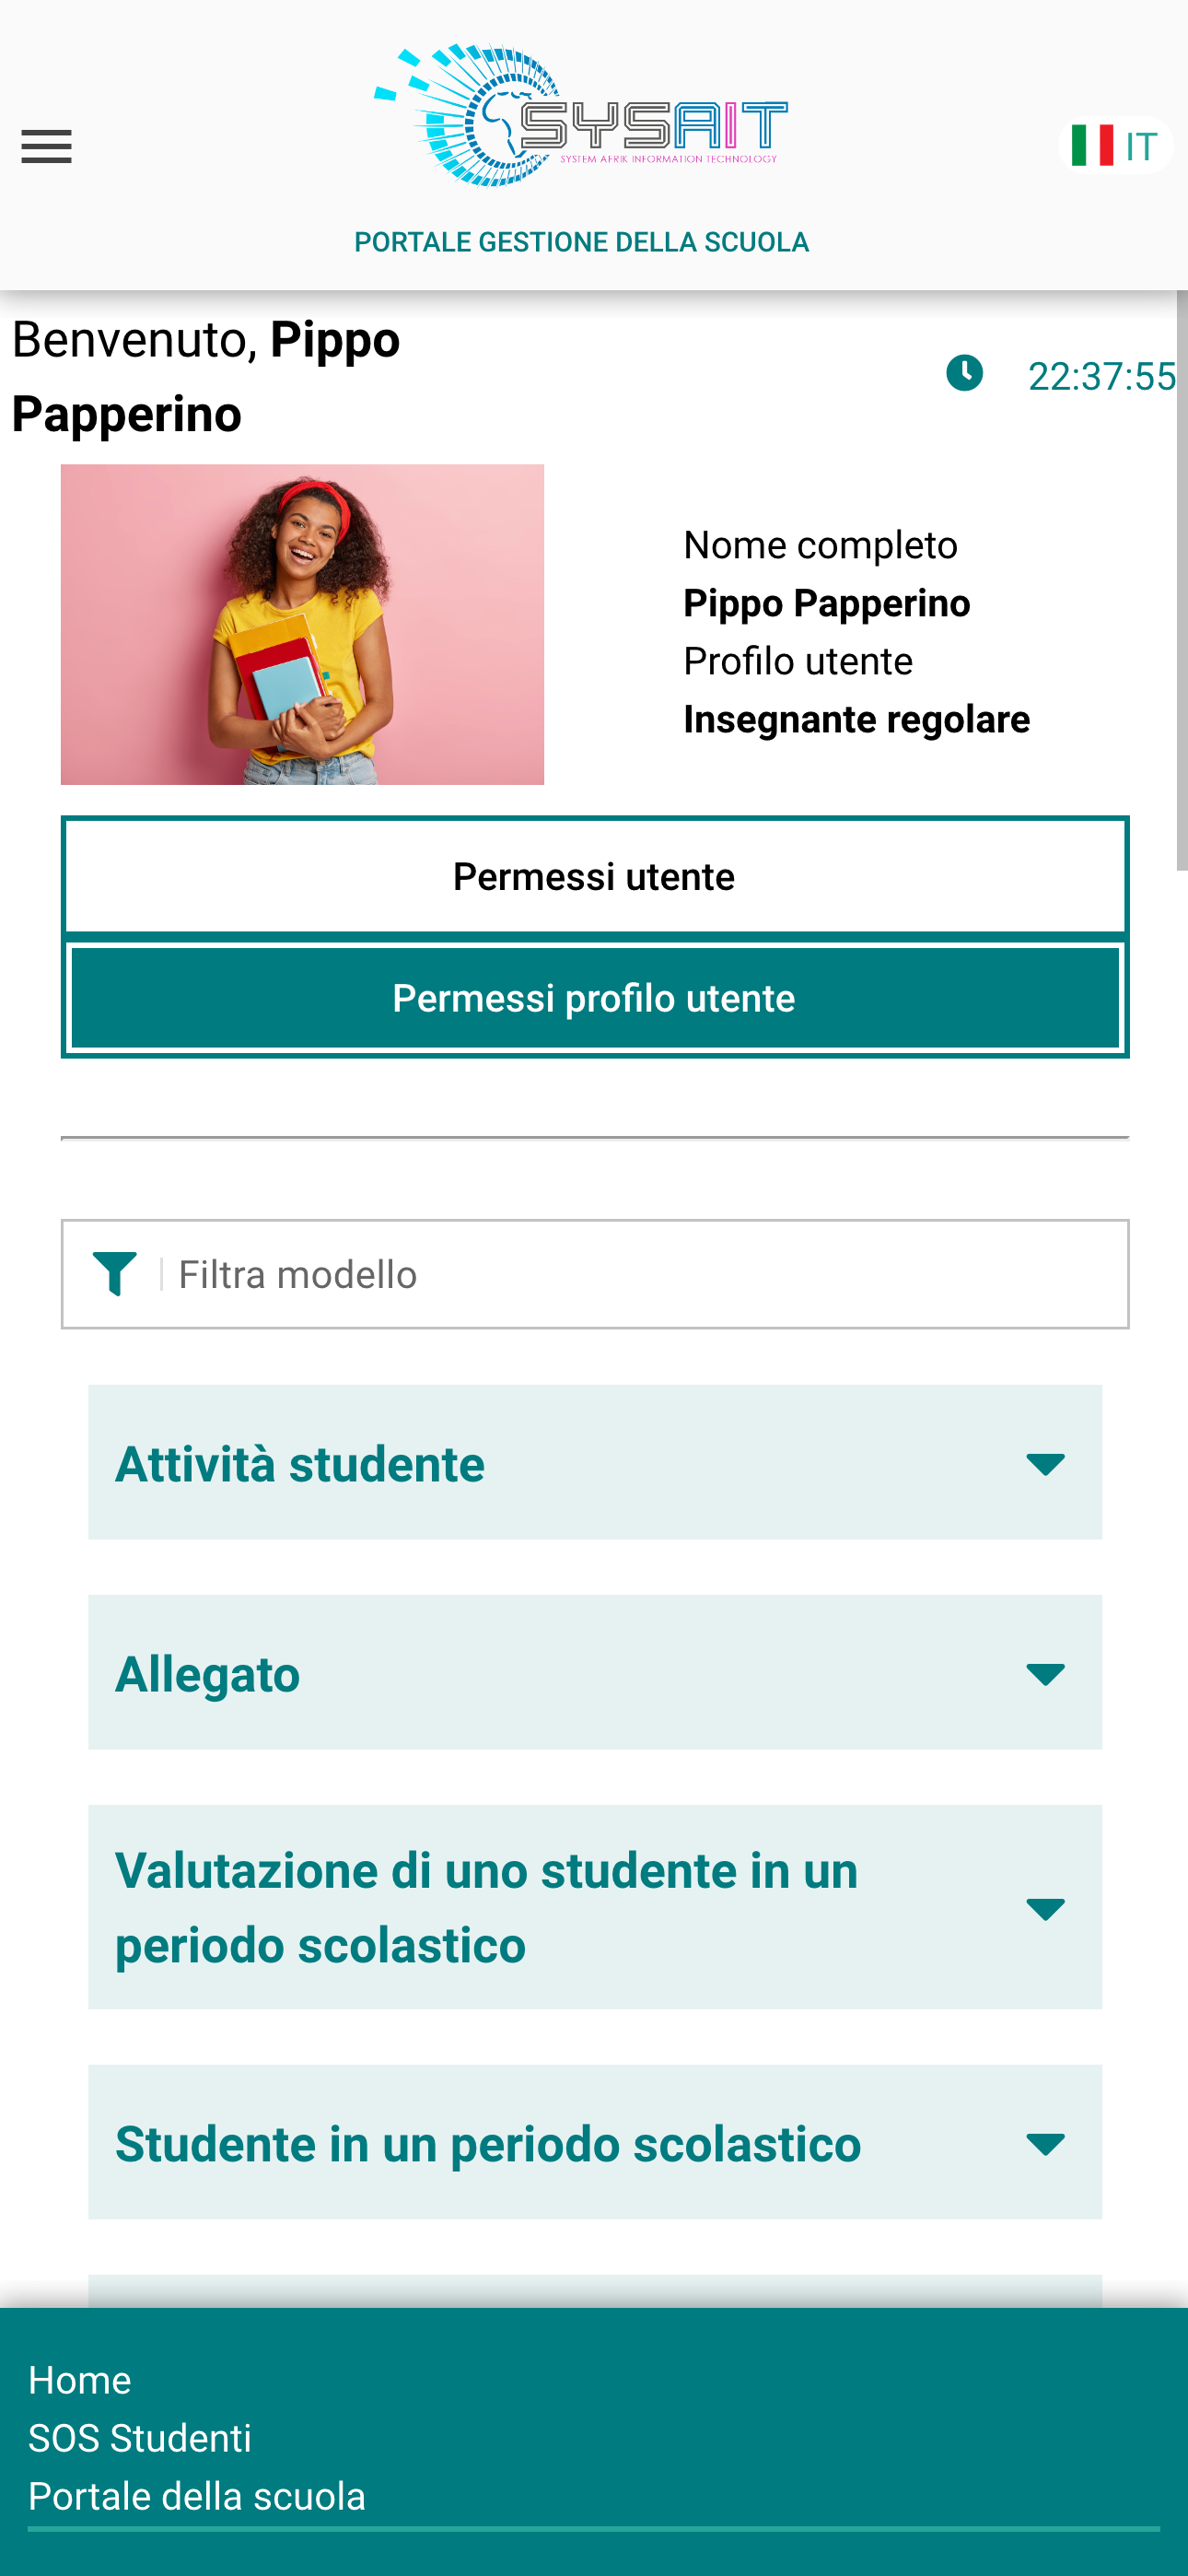
\includegraphics[width=0.9\textwidth]{../images/permission-management-mobile-profile.png}
			\end{figure}
		\end{column}
	\end{columns}
\end{frame}

\section{Test del frontend e del backend}

\begin{frame}{Test del frontend e del backend}
	\begin{columns}[T] % align columns at the top
		\begin{column}{0.5\textwidth}
			\textbf{Test del frontend}
			\begin{enumerate}
				\item \textbf{Jest}: framework di testing
				\item \textbf{Vue Test Utils}: libreria per testing dei componenti Vue.js
			\end{enumerate}
		\end{column}
		\begin{column}{0.5\textwidth}
			\textbf{Test del backend}
			\begin{enumerate}
				\item \textbf{Insomnia}: tool per verifica del corretto funzionamento delle chiamate
				\item \textbf{Test manuali}
			\end{enumerate}
		\end{column}
	\end{columns}
\end{frame}

\section{Implementazione in azione}
\begin{frame}{Implementazione in azione}
	\begin{center}
		%   \includemedia[
		%   	width=0.6\linewidth, % width of the media box
		%   	height=0.46\linewidth, % height of the media box
		%   	addresource=../images/modifica-permessi-eng.mov,
		%   	flashvars={
		%   			source=../images/modifica-permessi-eng.mov
		%   			&autoPlay=true
		%   			&loop=true
		%   		}
		%   ]{}{VPlayer.swf}
		 \href{https://youtu.be/P-cb9pAs8Go}{Demo su YouTube dell'implementazione}
	\end{center}
\end{frame}

\section{Conclusione}

\begin{frame}[fragile]{Conclusione}
	\begin{itemize}
		\item Requisiti funzionali e non funzionali raggiunti
		\item Interfaccia utente chiara e intuitiva, gestione semplice e immediata dei permessi
		\item Controllo granulare dei permessi per utenti e profili
		\item Integrazione con backend Ruby e database PostgreSQL
		\item Sistema scalabile e manutenibile
	\end{itemize}
\end{frame}

\begin{frame}[fragile]{Conclusione}
	\centering
	\Huge Grazie dell'attenzione
	\vfill
\end{frame}

\setbeamertemplate{background}{%
	\tikz[overlay,remember picture]%
	\node[opacity=0.8]at (current page.center)%
	{\includegraphics[width=.2\linewidth]%
		{example-image-a}};%
}

\end{document}
